\documentclass[../ClassicThesis.tex]{subfiles}
\begin{document}

%************************************************
\chapter{Approximation / Dimitri}\label{ch:appropximation}
%************************************************

\newcommand\myNotes[1]{\textcolor{red}{#1}}

\myNotes{TODO: Kurzer Zusammenfassender Absatz über das Kapitel}

\section{Mesh Simplification}

% Anfang Notizen ======================================================

% Übersicht:

% Welche Art von Simplification? -> Vertex Welding

% Was ist Vertex Welding?

% Warum brauchen wir Mesh Simplification?

% .



% .

% Alternative Methoden:

% Warum für Implementierung entschieden

% Ende Notizen ======================================================


Mesh simplification reduces the complexity of a {\threedmodel} by decreasing the amount of vertices and faces. In this process the original object gets approximated with less information while keeping the differences as low as possible. 

The used technique is known as 'vertex welding' in computer graphics: We merge two or more vertices that lie in a specified distance to each other. Therefore the mesh contains fewer vertices. As a consequence of the smaller vertex set thin faces no longer consist of three distinct vertices: Two nearby vertices are just represented by one vertex and the face gets deleted.

To illustrate the method the {\threedmodel} Stanford Bunny shown in Figure \ref{fig:origBunny} is simplified with an unusually high welding distance of 10mm in Figure \ref{fig:10mmBunny}. The images display each face with a different color to visualize the resulting face set. The loaded model consists of 8662 faces while the simplified bunny is reduced to 616 faces. Note how smaller details like eyes and ears get lost with higher welding distance while the overall shape still remains. (For effect illustration the welding distance is higher than the actual distance for processing)

\begin{figure}
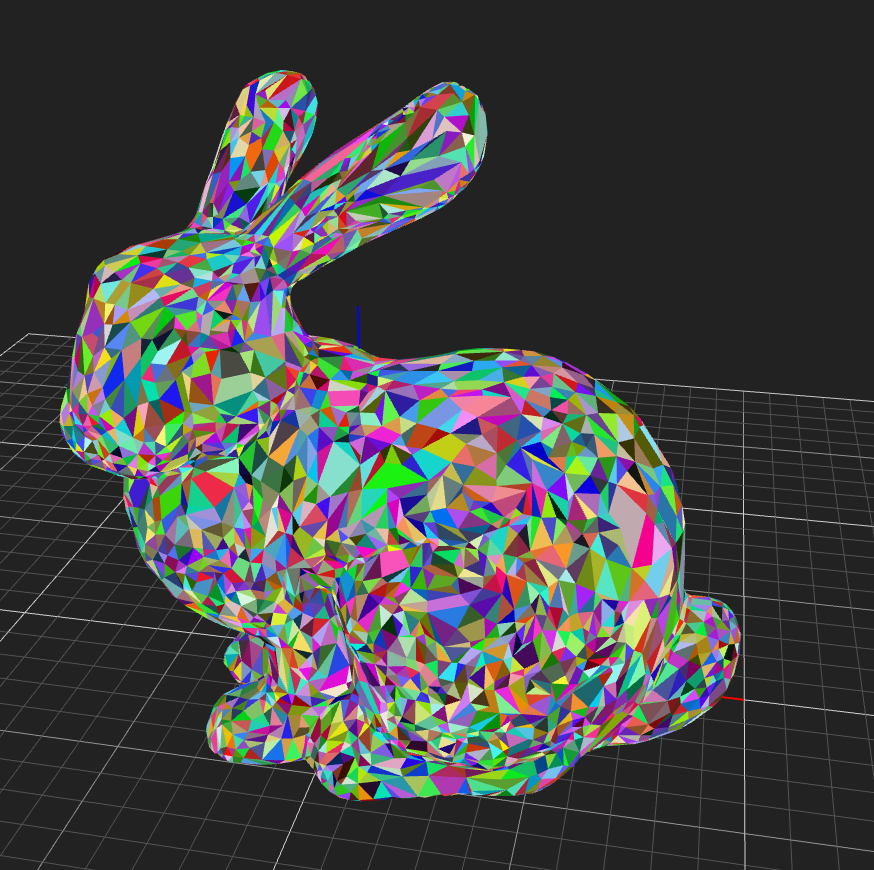
\includegraphics[width=0.8\columnwidth]{Images/04-approx-welding-rabbit-original.png}
\caption{Stanford Bunny with 8662 faces}
\label{fig:origBunny}
\end{figure}

\begin{figure}
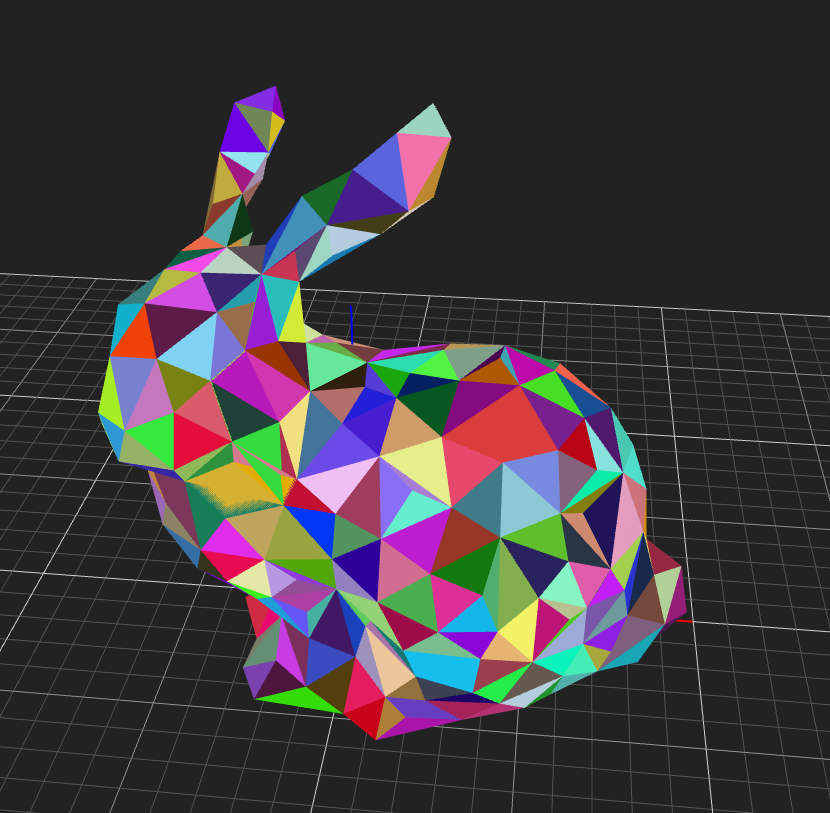
\includegraphics[width=0.8\columnwidth]{Images/04-approx-welding-rabbit-10mm.png}
\caption{Simplified Stanford Bunny with 616 faces (welding distance: 10mm)}
\label{fig:10mmBunny}
\end{figure}

Our mesh simplification tackles three issues:

\paragraph*{Processing Time}

After the model is loaded and stored we decrease its complexity to speed up following processing tasks. Every pipeline step benefits from this mesh simplification because of the reduced data they are working on which implicates a much faster pipeline runtime. 

\paragraph*{Abstraction}

Furthermore we eliminate beveled edges that are not functional but created by 3D-modeling software because of aesthetic reasons. The vertex welding approach gives us the needed shape abstraction to extract tiny details and minor curvatures we do not want to reproduce. 

\paragraph*{Elimination of redundant information created by our processing pipeline}

The algorithm can be reused in further processing to ensure unambiguous vertices that may occur due to rounding differences during transformations.



\subsection{Vertex Welding}

% Überblick

% 2 Modi -> preprocessed, first come


% Algorithmus erklären...


% Hase

% Beveled edges



Vertex Welding merges vertices and works as shown in Figure \ref{fig:vertex_welding}: 

A set of triangles is given. We choose a welding distance while points that lie further away of each other will not get merged. This is also the maximum distance a vertex can be moved from its original position. Therefore it describes the variance of input and resulting vertex set. 

For each cluster of vertices that get merged a new vertex is created (which is typically in the middle of all corresponding points). The original vertices are replaced by this new one in each triangle.

In case a triangle ($ABC$) has two points in the same merge cluster ($A$ and $B$) both get replaced by the new vertex $V$. As a result the triangle consists of the points $VVC$ while it does not contain three distinct vertices anymore - it is a line. If all three of its points lie in a cluster the outcome is a single point ($VVV$). In these cases the triangle gets deleted. The initial area of these deleted triangles is now covered by its adjacent triangles.

The result is an approximation of the input with fewer vertices and faces while the maximum variance equals the specified welding distance. As illustrated in Figure \ref{fig:vertex_welding} the resulting shape can also completely equal the original one without any differences: Only vertices inside the rectangle got merged which does not affect the outline of the object.


\begin{figure}
\includegraphics[width=1.0\columnwidth]{Images/04-approx-welding-overview.png}
% \includesvg{Images/04-approx-weldingoverview.svg}
\caption{Vertex Welding}
\label{fig:vertex_welding}
\end{figure}

\begin{figure}
\includegraphics[width=0.8\columnwidth]{Images/04-approx-welding-overview2.png}
\caption{Vertex Welding}
\label{fig:vertex_welding}
\end{figure}

\subsubsection{Usage}

For each welding application a new instance of \emph{VertexWelding} is created with the desired welding distance. Then the data can be preprocessed before the actual welding which provides the best possible result. Each vertex is then replaced by the \emph{VertexWelding} vertices. The points can be merged without preprocessing in case it is not needed (for instance while using very small welding distances). 

\emph{VertexWelding} provides 5 public functions:

\myNotes{ist 'public' das passende Wort?}

\myNotes{TODO: KLein-Großschreibung}

\begin{description}

\item[preProcessModel] \hfill \\
preprocesses the given meshlib model.

\item[preProcessVertices] \hfill \\
preprocesses the given array of vertices. A Vertex may be any object containing \emph{x}, \emph{y} and \emph{z} values.

\item[preProcessVertex] \hfill \\
preprocesses the given vertex which may be any object containing \emph{x}, \emph{y} and \emph{z} values.

\item[getCorrespondingVertex] \hfill \\
returns a new vertex based on the given one. This function is called for replacing each point of your object.

\item[replaceVerticesAndDeleteNonTriangularFaces] \hfill \\
handles the welding process for the given meshlib model: It replaces all vertices and deletes triangles that are not needed any more.

\end{description}

So if you want to weld a set of vertices, you can call \emph{preprocessVertices}, iterate over all points and replace them with the vertex from \emph{getCorrespondingVertex} or just replace them without preprocessing.

\subsubsection{Implementation}

\myNotes{TODO: Implementation}

\emph{VertexWelding} builds a list of weighted vertices during preprocessing. Each new vertex is either merged with an existing one or added to the list. A \emph{WeightedVertex} saves the number of represented points to merge new vertices correspondingly as shown in Figure \ref{fig:weightedVertex}. Then \emph{VertexWelding} returns the respective vertex for each requested point. 

In case a point is requested without preprocessing \emph{VertexWelding} builds its list without putting the new vertex in between the merged points but picks the first one as representative for all following.



\begin{figure}
\includegraphics[width=0.4\columnwidth]{Images/04-approx-WeightedVertex.png}
\caption{Resulting point (point 3) of welding a WeightedVertex with weight=2 (point 1) and point 2}
\label{fig:weightedVertex}
\end{figure}

\subsection{Simplification Pipelinestep}

After the pipeline step \emph{ModelStorage} saved the unmodified {\threedmodel} \emph{Simplification} provides a simplified version for all subsequent processing steps. It is directly followed by \emph{MeshSetup} and \emph{CoplanarFaces} which analyses the given mesh to combine multiple faces. 

This processing step serves two purposes: Removal of unwanted details and runtime improvement. Due to the capability of representing details with stacked plates, \emph{Simplification} is not run in \myNotes{StackedPlatesMethod (richtiger Name einzusetzen)}

\subsubsection{Details with stacked plates}

If sliced in an advantageous direction tiny details of a {\threedmodel} can be obtained with stacked plates. These details may be textures or bump maps like an engraving or a rough surface.

In general \emph{Simplification} removes such details as shown in Figure \ref{fig:3mmMakerbotMake}. With a welding distance of 3mm the result is a smooth surface while the original model shown in Figure \ref{fig:origMakerbotMake} contains the text 'Make:'.

To simplify a model without loosing such a text is not possible with the implemented vertex welding due to the nature of these texts: The labeled surface differs barely from a smooth surface. Therefore the vertices are so close to each other that welding will occur with every chosen welding distance. To obtain those texts the algorithm has to know areas where it must not weld. If you try to outline the text with a smaller welding distance there will always be some kind of artifacts: missing or degenerated letters like in Figure \ref{fig:08mmMakerbotMake}.

In order to be able to represent such texts with stacked plates \emph{Simplification} is not run in \myNotes{StackedPlatesMethod (richtiger Name einzusetzen)}

\myNotes{letzten Satz weglassen? steht ja schon vor dieser section...}

\begin{figure}
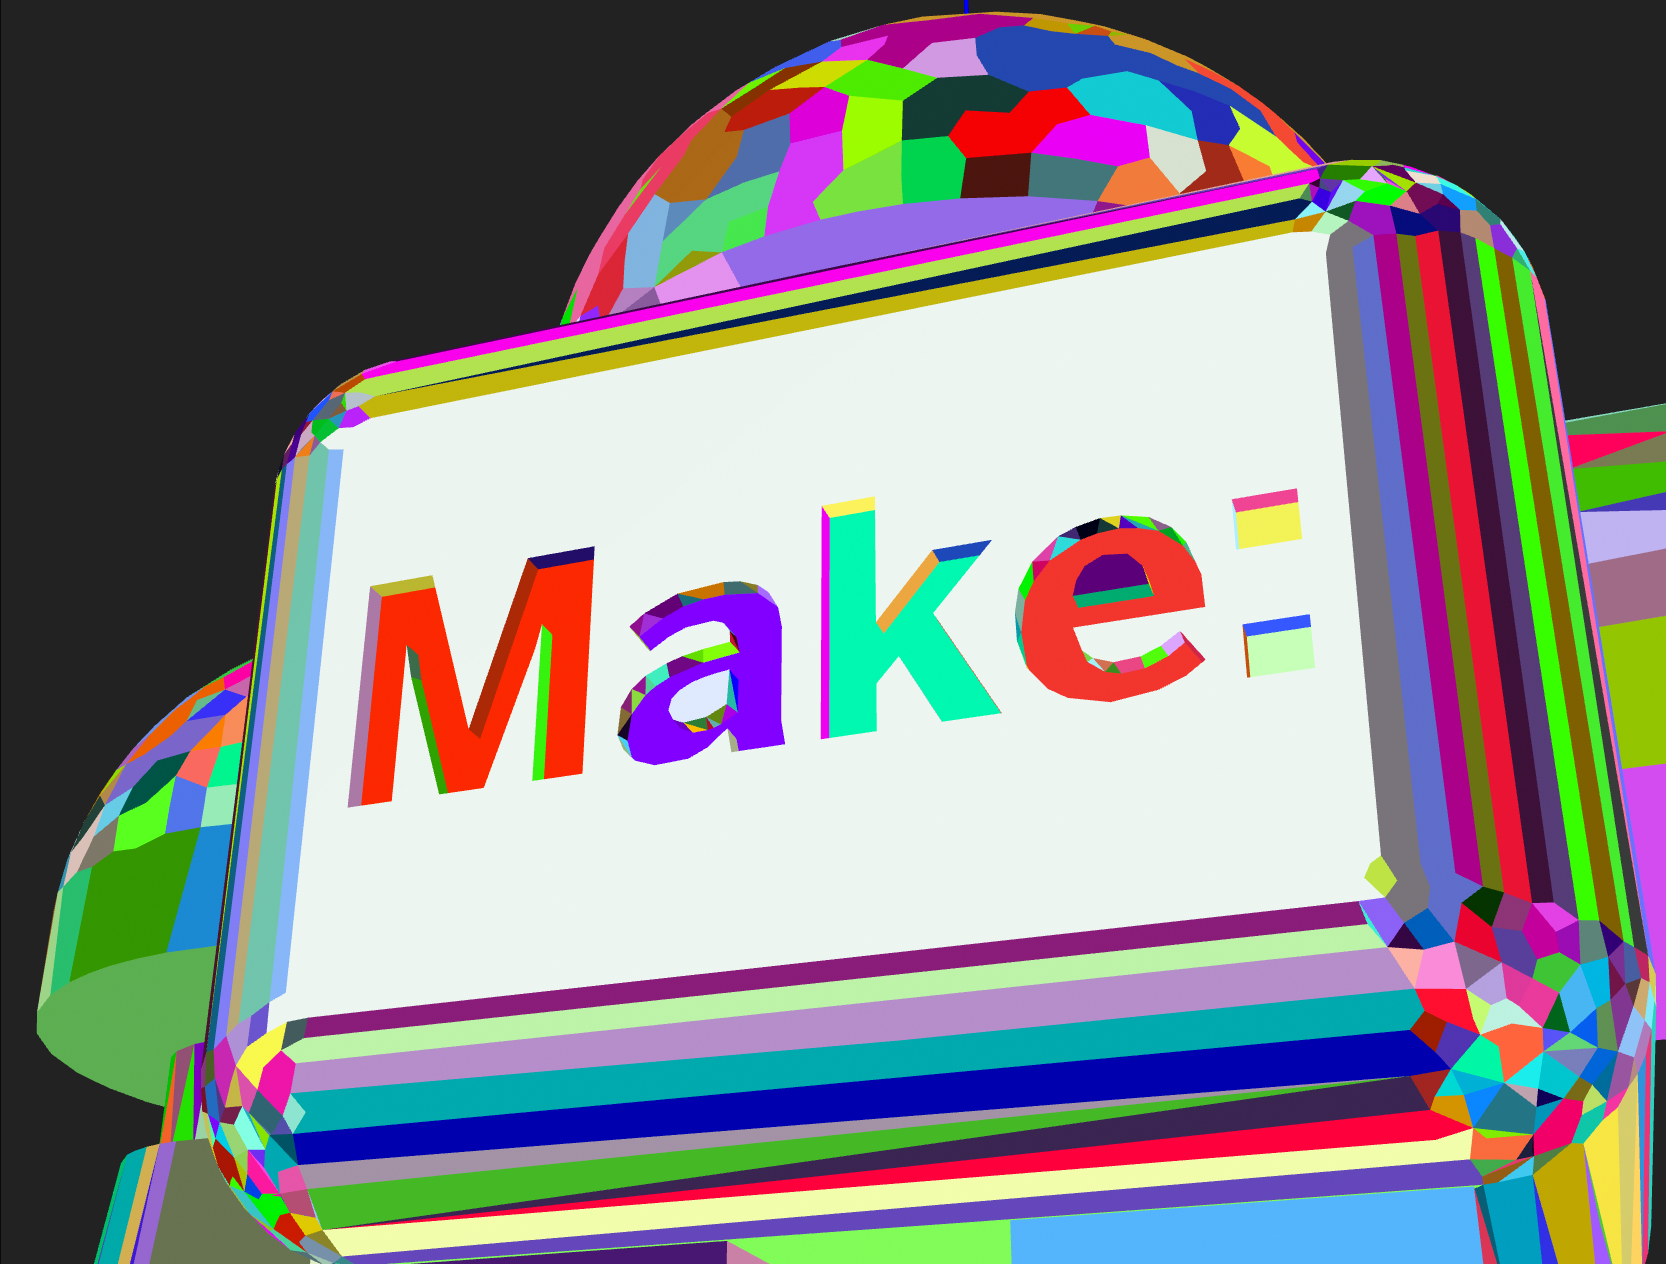
\includegraphics[width=0.8\columnwidth]{Images/04-approx-welding-make-unwelded.png}
\caption{Original Makerbot letters}
\label{fig:origMakerbotMake}
\end{figure}

\begin{figure}
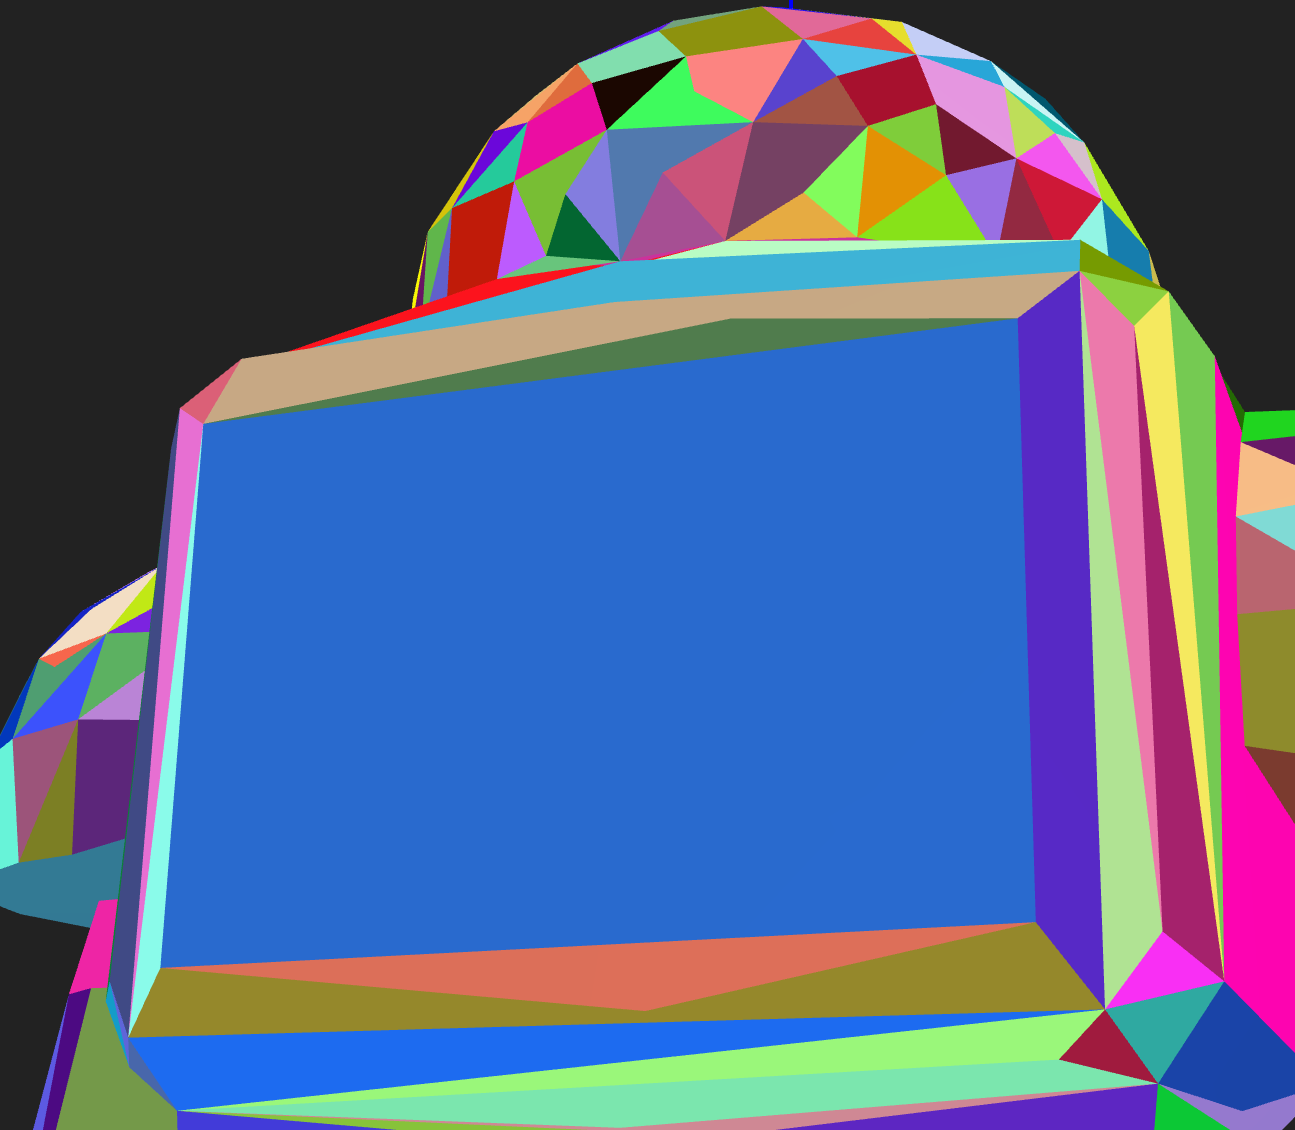
\includegraphics[width=0.8\columnwidth]{Images/04-approx-welding-make-3mm.png}
\caption{Simplified Makerbot with welding distance 3mm - letters completely removed}
\label{fig:3mmMakerbotMake}
\end{figure}

\begin{figure}
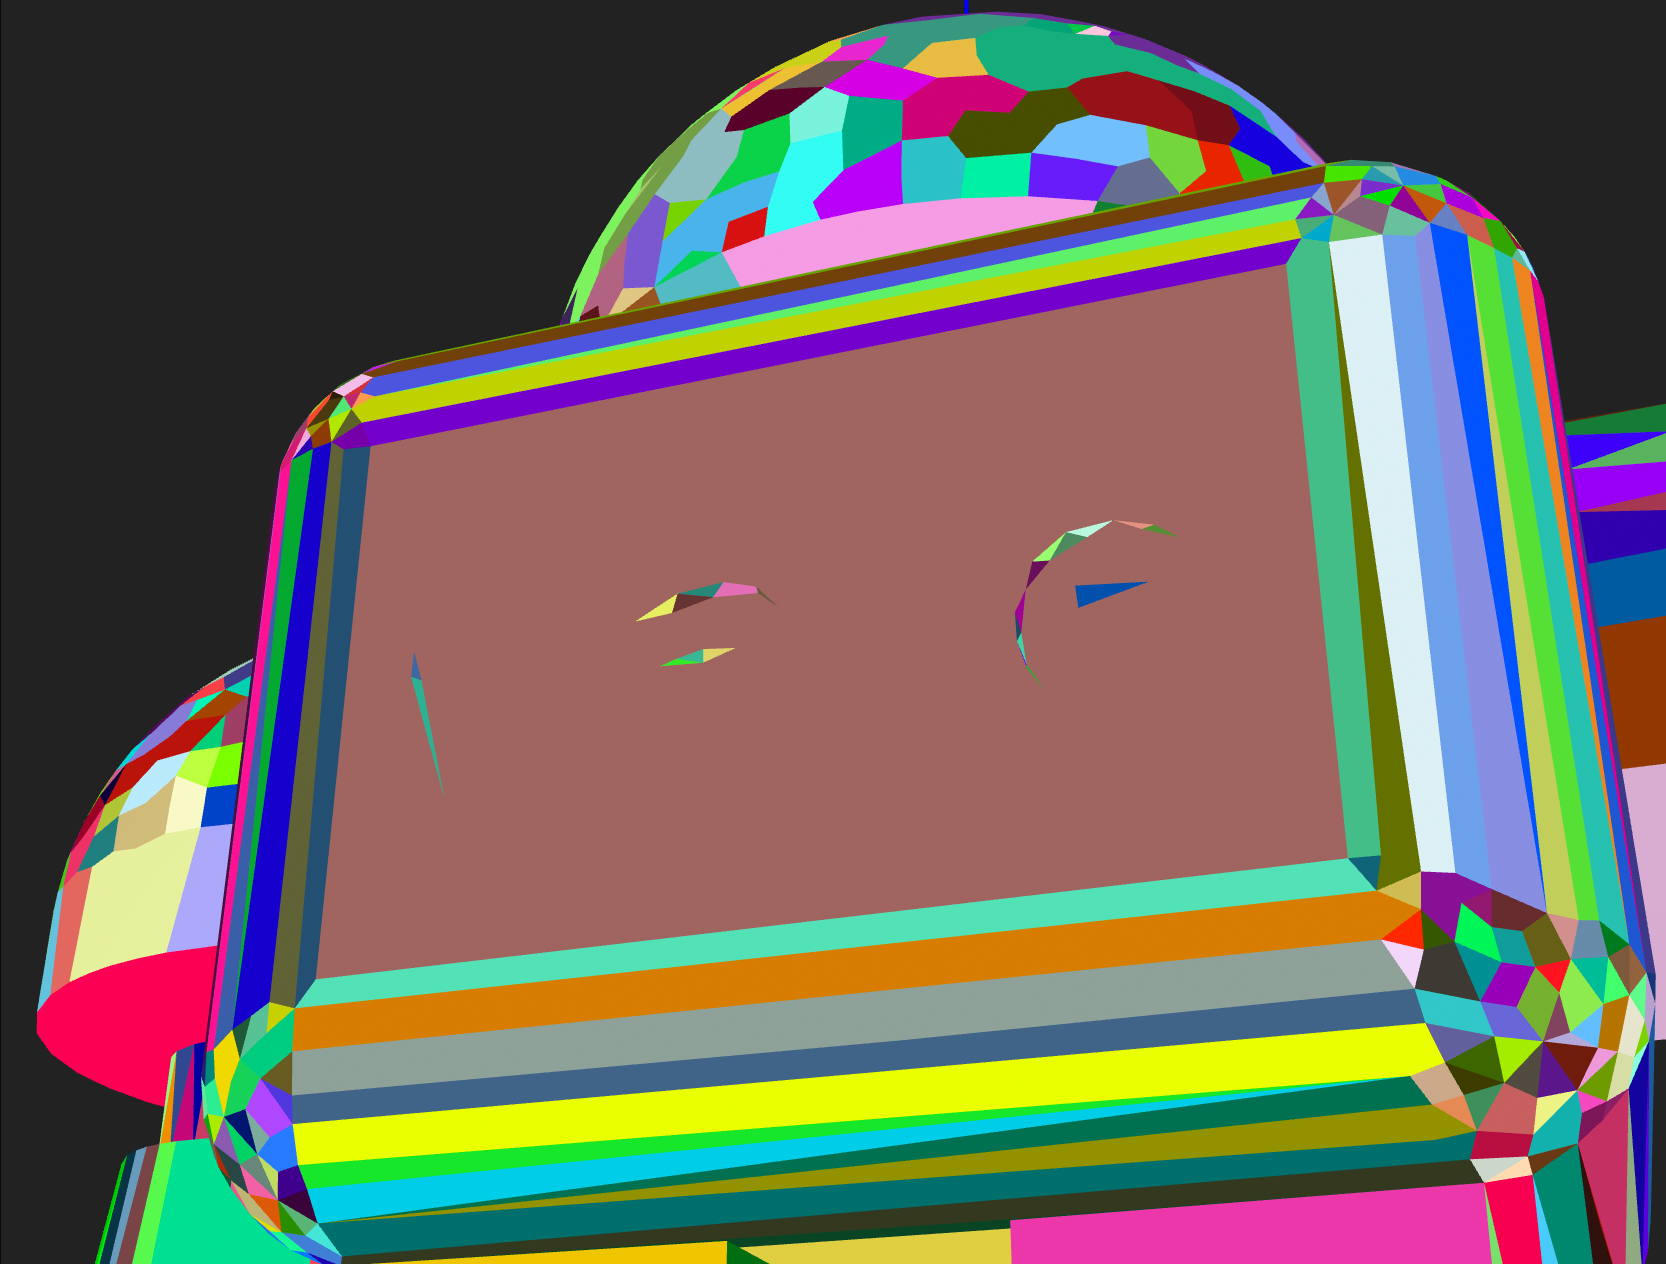
\includegraphics[width=0.8\columnwidth]{Images/04-approx-welding-make-0_8mm.png}
\caption{Simplified Makerbot with welding distance 0.8mm - artifacts}
\label{fig:08mmMakerbotMake}
\end{figure}

\subsubsection{Unwanted Details}

Most 3D editors offer to prettify objects by using curvatures instead of sharp edges. This can be done in various nuances to determine the smoothness of the curve.

Obviously it is much easier to reproduce two connected plates without a beveled edge in \myNotes{InherentPlates (richtiger Name einzusetzen)}. Since these curvatures are just for aesthetic reasons we revert the rounding without any loss of functionality.

Figure \ref{fig:beveled} shows three beveled cubes where the edge is subdivided into one, two and ten parts. All three result in the cube with straight edges after the \emph{Simplification}. The granularity of the created beveled edge does not make any difference for the outcome:
The higher the number of parts the denser the vertices while the absolute distance between start and end of a beveled edge remains the same. Therefore all vertices in this area get merged to the desired point independently from the edge segmentation.

In addition all sorts of surface modification like engravings and small attachments get removed which simplifies the plate recognition. In Figure \ref{fig:extruded_details} there is text on top of the actual surface and in Figure \ref{fig:pushed_in_details} there is text pushed into the surface while both text is removed in the resulting object.

\myNotes{statt an "extruded details" lieber an makerbot von vorher erklären?}

\begin{figure}
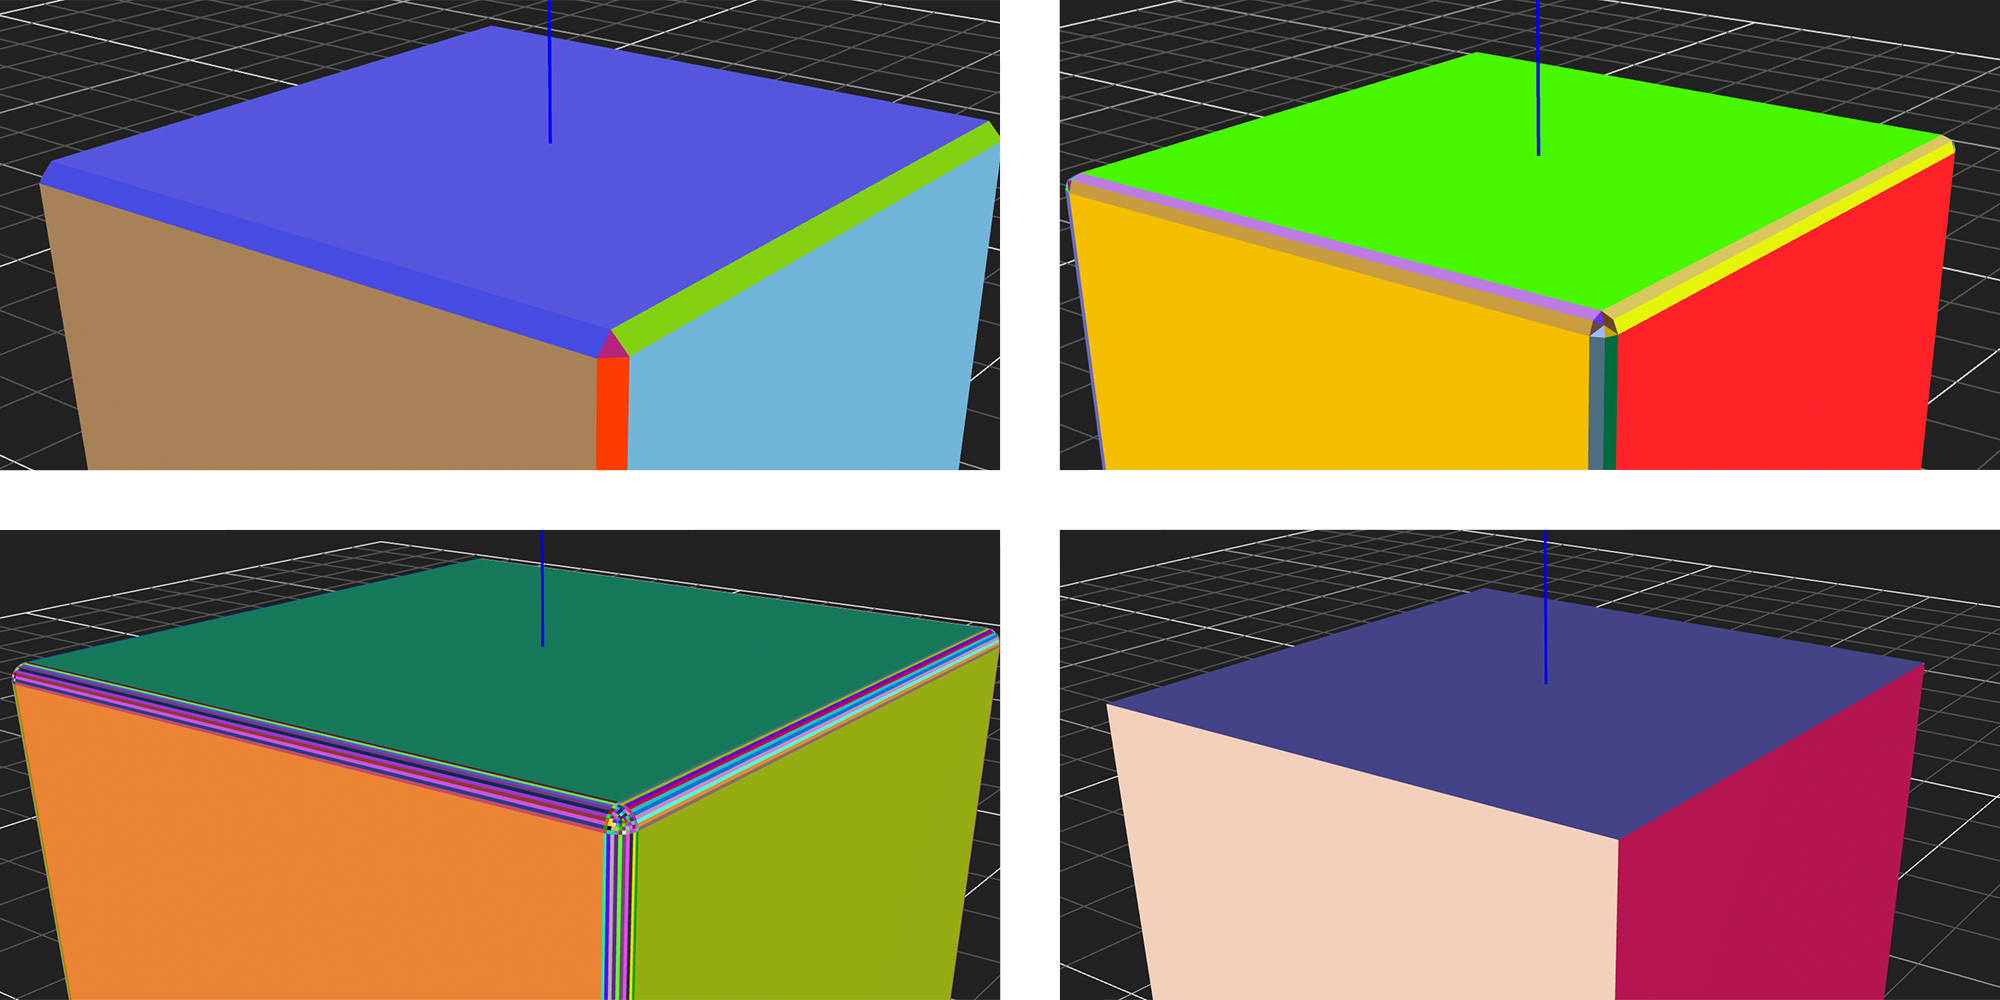
\includegraphics[width=1.0\columnwidth]{Images/04-approx-welding-beveled.png}
\caption{Beveled cube with 1, 2, 10 subdivisions and their resulting cube without beveled edges}
\label{fig:beveled}
\end{figure}

\begin{figure}
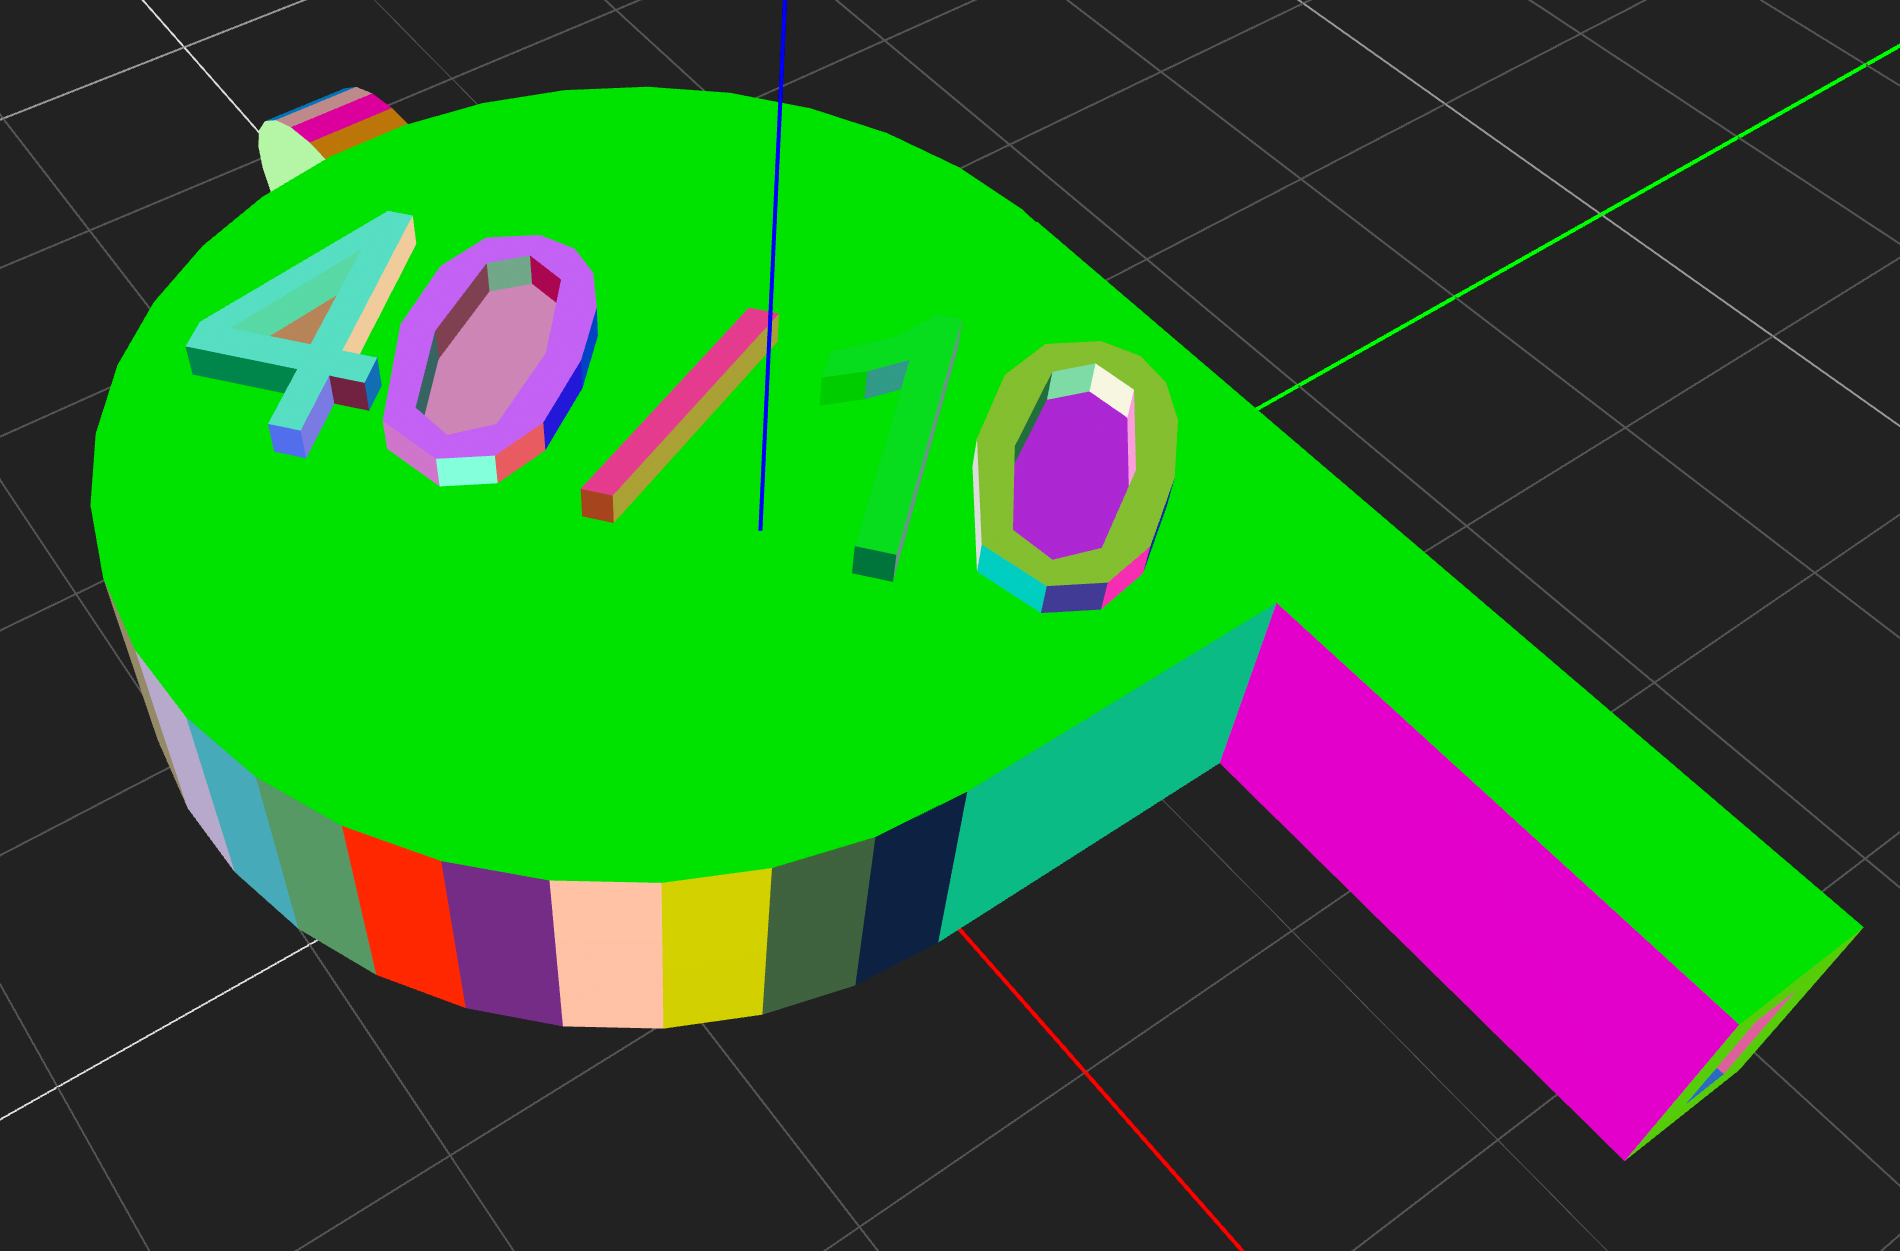
\includegraphics[width=0.5\columnwidth]{Images/04-approx-welding-beveled-extruded.png}
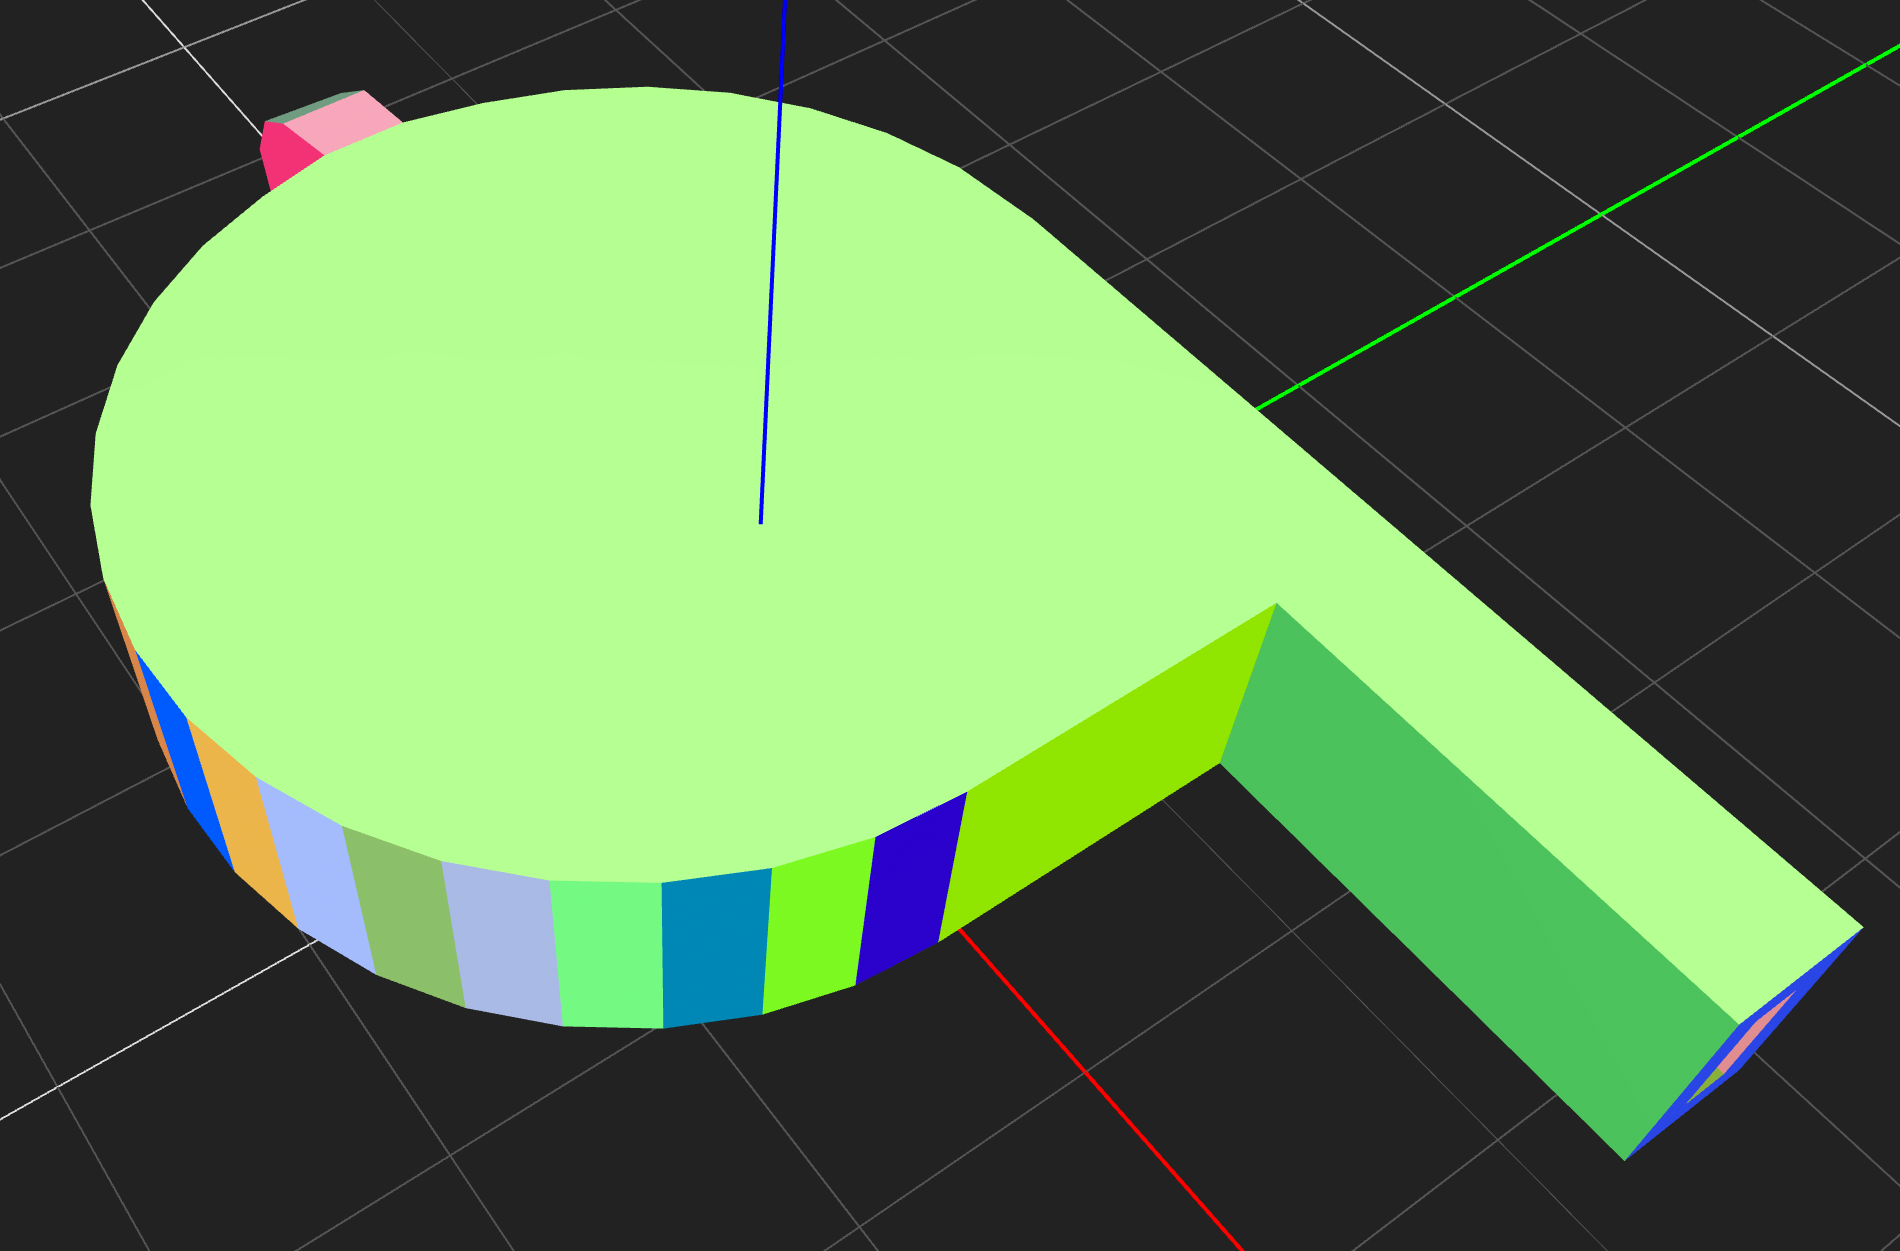
\includegraphics[width=0.5\columnwidth]{Images/04-approx-welding-beveled-extruded-result.png}
\caption{Extruded details}
\label{fig:extruded_details}
\end{figure}

\begin{figure}
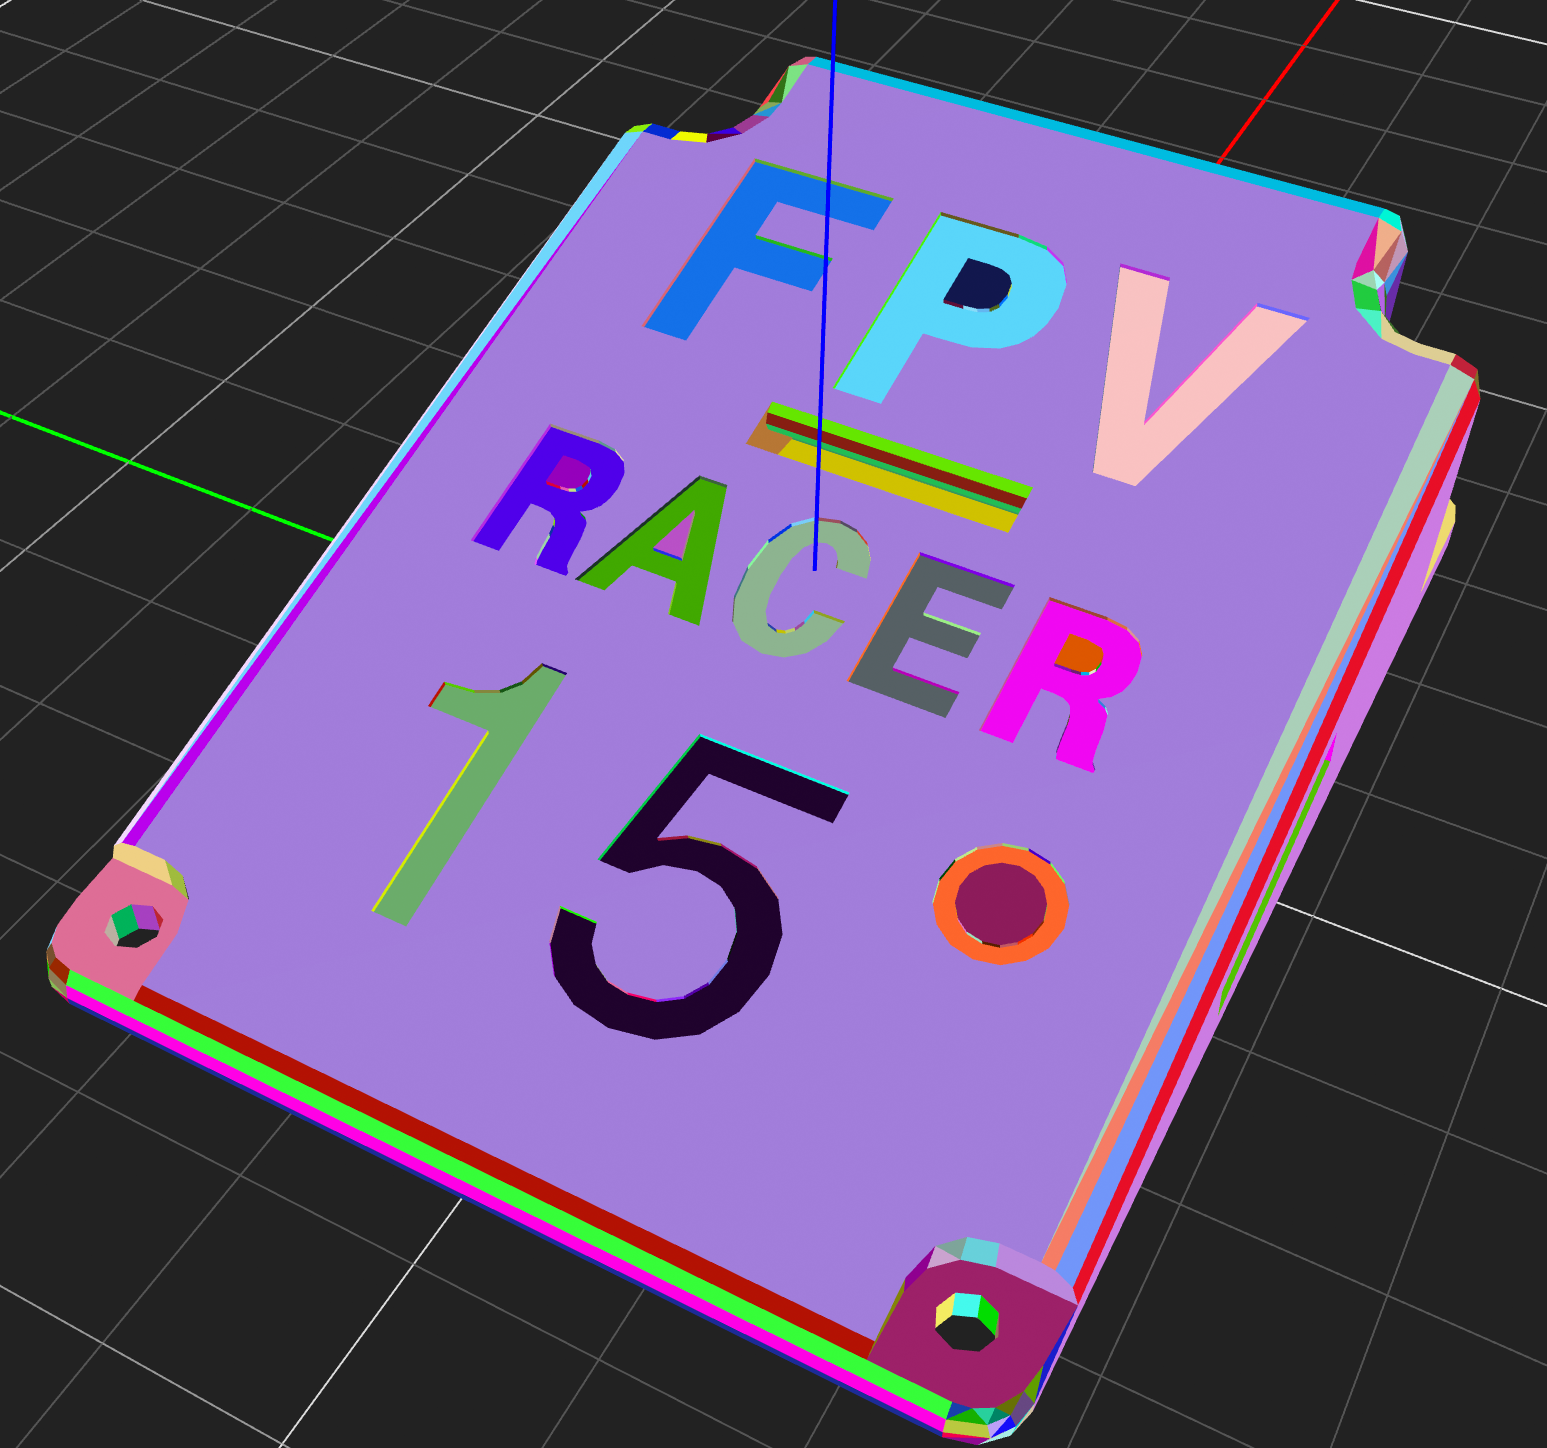
\includegraphics[width=0.5\columnwidth]{Images/04-approx-welding-pushedIn.png}
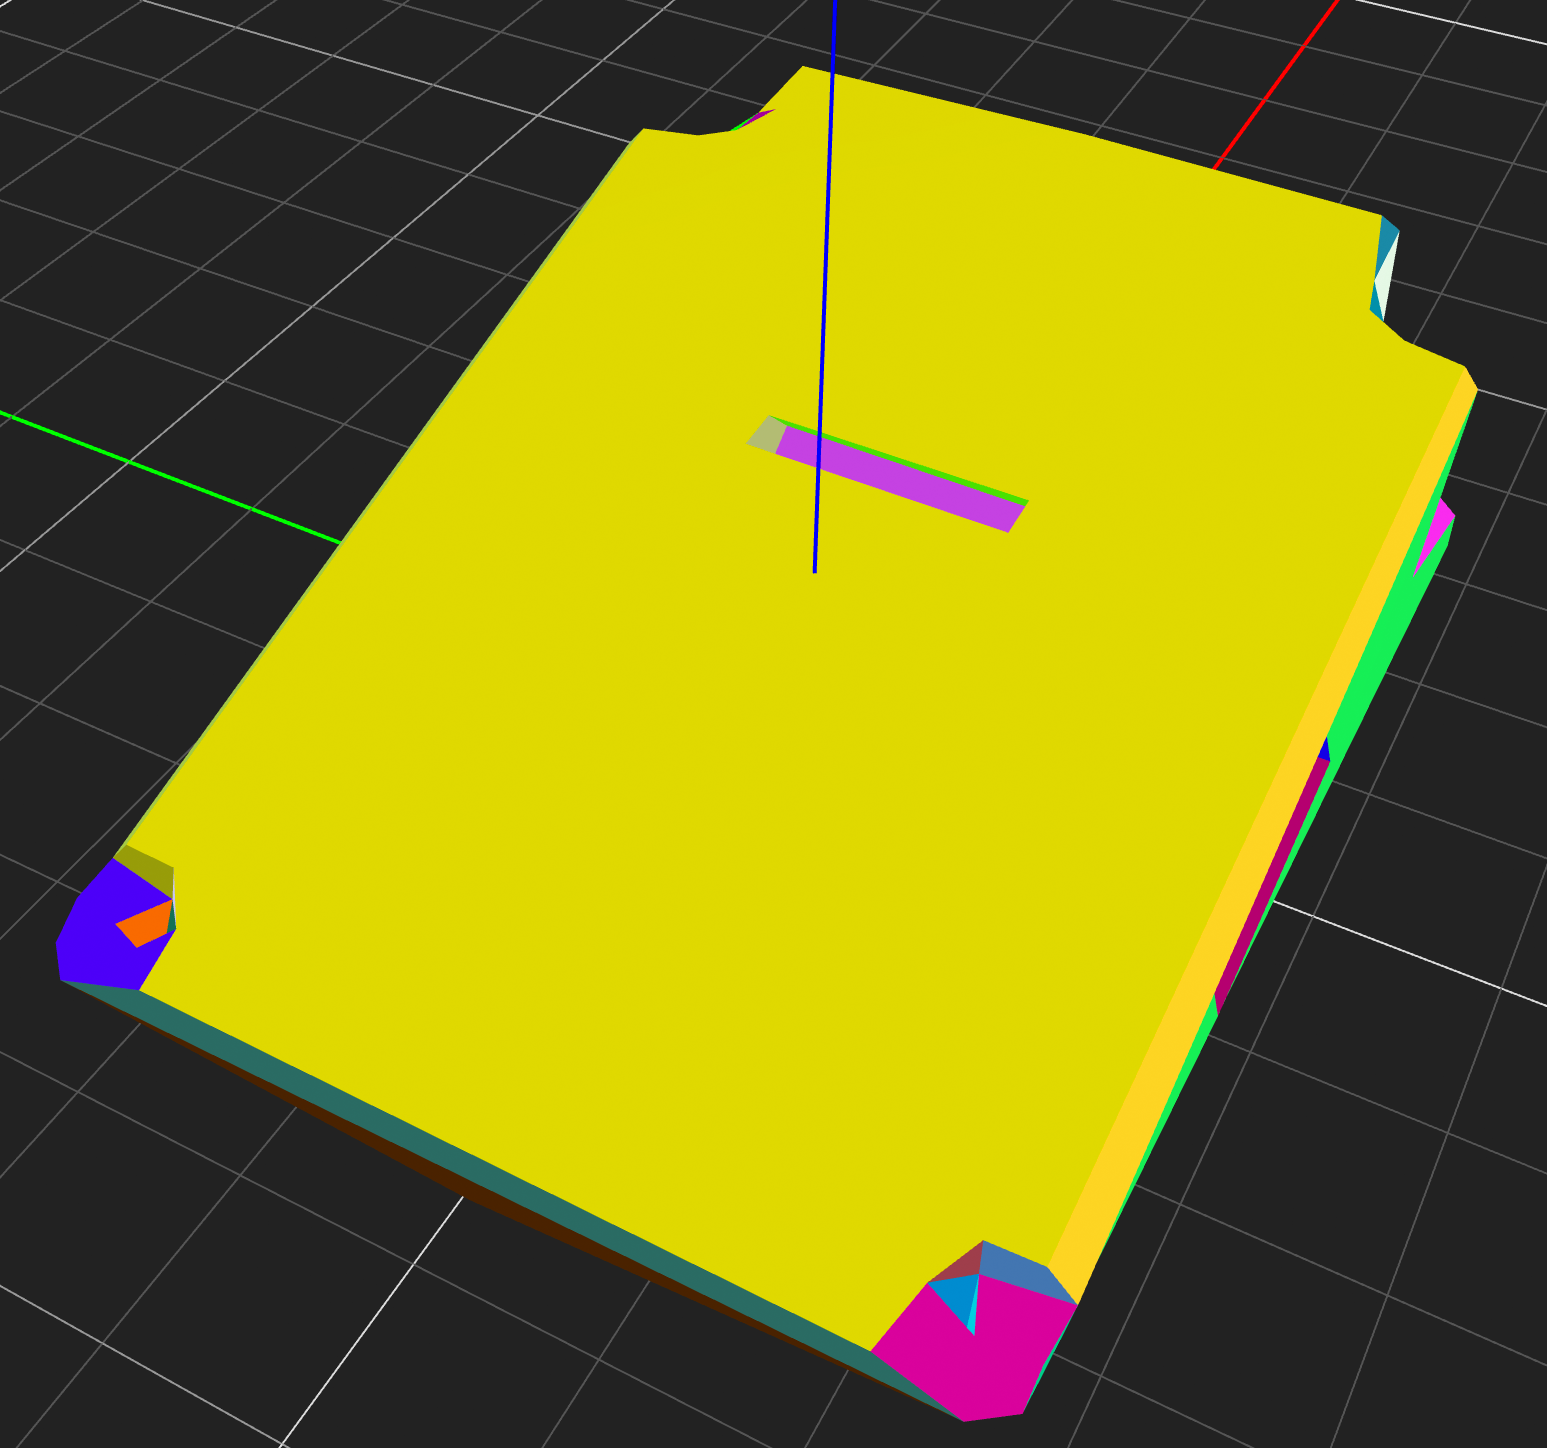
\includegraphics[width=0.5\columnwidth]{Images/04-approx-welding-pushedIn-result.png}
\caption{Pushed in details}
\label{fig:pushed_in_details}
\end{figure}


\subsubsection{Processing Time Improvement}

\myNotes{TODO: processing time improvement}

\myNotes{TODO: Zahlen Runtime Vergleich: mit und ohne Simplification}

\subsubsection{Process}

The pipeline step clones the model due to our immutable state approach so the original model can be accessed at any point in time.

\myNotes{immutable state approach sollte in Kap. Architecture erklärt sein}

\paragraph{Welding Distance}

\myNotes{TODO: Kompletter Abschnitt "Welding Distance" neu schreiben, da leicht obsolet}

\myNotes{TODO: calculation of welding distance}

The user can modify the welding distance in the UI element shown in Figure \ref{fig:weldingUI}. This is necessary to support extreme {\threedmodel}s and adapt to their specialties. For instance both tiny models that span only a few millimeters and huges ones where a stronger simplification would be beneficial.

\myNotes{TODO: change ui text}

\begin{figure}
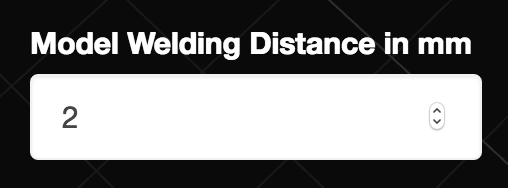
\includegraphics[width=0.5\columnwidth]{Images/04-approx-weldingUI.png}
\caption{Vertex Welding UI Element}
\label{fig:weldingUI}
\end{figure}

The value gets updated in the global config file which will be used in the next recomputation. The default is 2mm which works perfect for most {\threedmodel}s and removes all beveled edges created by common editors like Blender\footnote{https://www.blender.org}. Due to the nature of beveled edges all methods only modify small areas around corners which results in dense vertices that get merged by our vertex welding. 

\myNotes{TODO: no config??}

\myNotes{TODO: Zahlen - 2mm perfekt für x von y modellen}

\paragraph{Welding}

At first all vertices get preprocessed by the welding algorithm to create the vertex lookup-table. After that the model is passed to \emph{VertexWelding} which iterates over all faces to replace its vertices with their corresponding vertex from the preprocessed table. Meanwhile it checks for invalid faces and deletes them.

\paragraph{Provided Model}

After the actual vertex welding the {\threedmodel} is checked for an empty face set which might occur if the user picked a large welding distance. In this case the stored and unmodified mesh is returned in order to run the rest of the pipeline. The user gets reminded to pick a better welding distance.

The mesh preparation itself is extracted into another pipeline step: \emph{MeshSetup}. It takes the simplified {\threedmodel} and makes it ready for all further processing: face vertex mesh building, normal calculation and mesh indexing.


    
\subsection{Reusage for redundant information elimination}

The algorithm can be reused in later processing steps whenever we want to ensure that a vertex is not split into multiple ones that lie close together. 

For instance, this may occur in \myNotes{CurvedShapes (richtige Bezeichnung einzusetzen)} where \emph{VertexWelder} is used to eliminate these point cluster. In general whenever a new form or object is created (as well in 3D as in 2D) welding can be applied to ensure unambiguous points. Otherwise these vertices may be scattered due to rounding differences during rotation or other transformations: If you have one vertex in two different objects and the objects get transformed in different ways the resulting vertex of each object may slightly differ because of floating inaccuracies.

\myNotes{TODO: letzten Satz besser schreiben}


\subsection{Alternative Methoden}

\subsection{Warum diese Methode gewählt?}

\section{Point on Line Removal}

\section{vllt: Remove Contained Plates - in Lukas Kapitel}

\section{Prism Classifier - in Classifier Kapitel}

\section{Hole Detection - in Plates Kapitel}

% (Plate) - Shape - EdgeLoop - Architektur und Funktionalität
% (Clipping)

\end{document}